\documentclass[14pt]{beamer}
%%%%%%%%%%%%%%%%%%%%%%%%%%%%%%%%%%%%%%%%%%%%%%%%%%%%%%%%%%%%%
% Meta informations:
\newcommand{\trauthor}{Weipeng He}
\newcommand{\trtype}{Seminar} %{Proseminar} %{Seminar} %{Workshop}
\newcommand{\trcourse}{Bio-inspired Artificial Intelligence}
\newcommand{\trtitle}{Self-replicating Robots : A review}
\newcommand{\trmatrikelnummer}{6411529}
\newcommand{\tremail}{2he@informatik.uni-hamburg.de}
\newcommand{\trinstitute}{Department of Informatics}
\newcommand{\trwebsiteordate}{6 February, 2013}

%%%%%%%%%%%%%%%%%%%%%%%%%%%%%%%%%%%%%%%%%%%%%%%%%%%%%%%%%%%%%
% Languages:

% Falls die Ausarbeitung in Deutsch erfolgt:
% \usepackage[german]{babel}
% \usepackage[T1]{fontenc}
% \usepackage[latin1]{inputenc}
% \usepackage[latin9]{inputenc}	 				
% \selectlanguage{german}

% If the thesis is written in English:
\usepackage[english]{babel} 						
\selectlanguage{english}

%%%%%%%%%%%%%%%%%%%%%%%%%%%%%%%%%%%%%%%%%%%%%%%%%%%%%%%%%%%%%
% Bind packages:
\usepackage{beamerthemesplit}
\usetheme{Boadilla}
%\usetheme{Copenhagen}
%\usetheme{Darmstadt}
%\usetheme{Frankfurt}
%\usetheme{Ilmenau}
%\usetheme{JuanLesPins}
%\usetheme{Madrid}
%\usetheme{Warsaw }
%\usecolortheme{dolphin}
%\setbeamertemplate{sections/subsections in toc}[sections numbered]
%\beamertemplatenavigationsymbolsempty
%\setbeamertemplate{headline}[default] 	% deaktiviert die Kopfzeile
\setbeamertemplate{navigation symbols}{}% deaktiviert Navigationssymbole
%\useinnertheme{rounded}

\usepackage{acronym}                    % Acronyms
\usepackage{algorithmic}								% Algorithms and Pseudocode
\usepackage{algorithm}									% Algorithms and Pseudocode
\usepackage{amsfonts}                   % AMS Math Packet (Fonts)
\usepackage{amsmath}                    % AMS Math Packet
\usepackage{amssymb}                    % Additional mathematical symbols
\usepackage{amsthm}
\usepackage{color}                      % Enables defining of colors via \definecolor
\usepackage{fancybox}                   % Gleichungen einrahmen
\usepackage{fancyhdr}										% Paket zur schickeren der Gestaltung der 
\usepackage{graphicx}                   % Inclusion of graphics
%\usepackage{latexsym}                  % Special symbols
\usepackage{longtable}									% Allow tables over several parges
\usepackage{listings}                   % Nicer source code listings
\usepackage{lmodern}
\usepackage{multicol}										% Content of a table over several columns
\usepackage{multirow}										% Content of a table over several rows
\usepackage{rotating}										% Alows to rotate text and objects
%\usepackage[section]{placeins}          % Ermoeglich \Floatbarrier fuer Gleitobj. 
\usepackage[hang]{subfigure}            % Allows to use multiple (partial) figures in a fig
%\usepackage[font=footnotesize,labelfont=rm]{subfig}	% Pictures in a floating environment
\usepackage{tabularx}										% Tables with fixed width but variable rows
\usepackage{url,xspace,boxedminipage}   % Accurate display of URLs

\definecolor{uhhRed}{RGB}{254,0,0}		  % Official Uni Hamburg Red
\definecolor{uhhGrey}{RGB}{136,136,136} % Official Uni Hamburg Grey
\definecolor{uhhLightGrey}{RGB}{180,180,180} % Official Uni Hamburg LightGrey
\definecolor{uhhLightLightGrey}{RGB}{220,220,220} % Official Uni Hamburg LightLightGrey
\setbeamertemplate{itemize items}[ball]
\setbeamercolor{title}{fg=uhhRed,bg=white}
\setbeamercolor{title in head/foot}{bg=uhhRed}
\setbeamercolor{block title}{bg=uhhGrey,fg=white}
\setbeamercolor{block body}{bg=uhhLightLightGrey,fg=black}
\setbeamercolor{section in head/foot}{bg=black}
\setbeamercolor{frametitle}{bg=white,fg=uhhRed}
\setbeamercolor{author in head/foot}{bg=black,fg=white}
\setbeamercolor{author in footline}{bg=white,fg=black}
\setbeamercolor*{item}{fg=uhhRed}
\setbeamercolor*{section in toc}{fg=black}
\setbeamercolor*{separation line}{bg=black}
\setbeamerfont*{author in footline}{size=\scriptsize,series=\mdseries}
\setbeamerfont*{institute}{size=\footnotesize}

\newcommand{\opticalseperator}{0.0025\paperwidth}

\institute{Universit\"at Hamburg\\\trinstitute}
\title{\trtitle}
\subtitle{\trtype}
\author{\trauthor}
\date{}
\logo{}

%%%%%%%%%%%%%%%%%%%%%%%%%%%%%%%%%%%%%%%%%%%%%%%%%%%%%%%%%%%%%
% Configurationen:
% \hypersetup{pdfpagemode=FullScreen}

\hyphenation{whe-ther} 									% Manually use: "\-" in a word: Staats\-ver\-trag

%\lstloadlanguages{C}                   % Set the default language for listings
\DeclareGraphicsExtensions{.pdf,.svg,.jpg,.png,.eps} % first try pdf, then eps, png and jpg
\graphicspath{{./data/}} 								% Path to a folder where all pictures are located

%%%%%%%%%%%%%%%%%%%%%%%%%%%%
% Costom Definitions:
\setbeamertemplate{title page}
{
  \vbox{}
	\vspace{0.4cm}
  \begin{centering}
    \begin{beamercolorbox}[sep=8pt,center,colsep=-4bp]{title}
      \usebeamerfont{title}\inserttitle\par%
      \ifx\insertsubtitle\@empty%
      \else%
        \vskip0.20em%
        {\usebeamerfont{subtitle}\usebeamercolor[fg]{subtitle}\insertsubtitle\par}%
      \fi%     
    \end{beamercolorbox}%
		\vskip0.4em
    \begin{beamercolorbox}[sep=8pt,center,colsep=-4bp,rounded=true,shadow=true]{author}
      \usebeamerfont{author}\insertauthor \\ \insertinstitute
    \end{beamercolorbox}

	  \vfill
% 	  \begin{beamercolorbox}[ht=8ex,center]{}
% 		  
\includegraphics[width=0.20\paperwidth]{wtmIcon.pdf}
% 	  \end{beamercolorbox}%
    \begin{beamercolorbox}[sep=8pt,center,colsep=-4bp,rounded=true,shadow=true]{institute}
      \usebeamerfont{institute}\trwebsiteordate
    \end{beamercolorbox}
		\vspace{-0.1cm}
  \end{centering}
}

\setbeamertemplate{frametitle}
{
\begin{beamercolorbox}[wd=\paperwidth,ht=3.8ex,dp=1.2ex,leftskip=0pt,rightskip=4.0ex]{frametitle}%
		\usebeamerfont*{frametitle}\centerline{\insertframetitle}
	\end{beamercolorbox}
	\vspace{0.0cm}
}

\setbeamertemplate{footline}
{
  \leavevmode
	\vspace{-0.05cm}
  \hbox{
	  \begin{beamercolorbox}[wd=.32\paperwidth,ht=4.8ex,dp=2.7ex,center]{author in footline}
	    \hspace*{2ex}\usebeamerfont*{author in footline}\trauthor
	  \end{beamercolorbox}%
	  \begin{beamercolorbox}[wd=.60\paperwidth,ht=4.8ex,dp=2.7ex,center]{author in footline}
	    \usebeamerfont*{author in footline}\trtitle
	  \end{beamercolorbox}%
	  \begin{beamercolorbox}[wd=.07\paperwidth,ht=4.8ex,dp=2.7ex,center]{author in footline}
	    \usebeamerfont*{author in footline}\insertframenumber{}
	  \end{beamercolorbox}
  }
	\vspace{0.15cm}
}

%%%%%%%%%%%%%%%%%%%%%%%%%%%%
% Additional 'theorem' and 'definition' blocks:
\newtheorem{axiom}{Axiom}[section] 	
%\newtheorem{axiom}{Fakt}[section]			% Wenn in Deutsch geschrieben wird.
%Usage:%\begin{axiom}[optional description]%Main part%\end{fakt}

%Additional types of axioms:
\newtheorem{observation}[axiom]{Observation}

%Additional types of definitions:
\theoremstyle{remark}
%\newtheorem{remark}[section]{Bemerkung} % Wenn in Deutsch geschrieben wird.
\newtheorem{remark}[section]{Remark} 

%%%%%%%%%%%%%%%%%%%%%%%%%%%%
% Provides TODOs within the margin:
\newcommand{\TODO}[1]{\marginpar{\emph{\small{{\bf TODO: } #1}}}}

%%%%%%%%%%%%%%%%%%%%%%%%%%%%
% Abbreviations and mathematical symbols
\newcommand{\modd}{\text{ mod }}
\newcommand{\RS}{\mathbb{R}}
\newcommand{\NS}{\mathbb{N}}
\newcommand{\ZS}{\mathbb{Z}}
\newcommand{\dnormal}{\mathit{N}}
\newcommand{\duniform}{\mathit{U}}

\newcommand{\erdos}{Erd\H{o}s}
\newcommand{\renyi}{-R\'{e}nyi}

%%%%%%%%%%%%%%%%%%%%%%%%%%%%
% Provides latin abbriviations:
\newcommand{\etal}{\textit{et al.}}
\newcommand{\etc}{\textit{etc.}}
\newcommand{\eg}{\textit{e.g.}}

%%%%%%%%%%%%%%%%%%%%%%%%%%%%
% Display of TOCs:
% \AtBeginSection[]
% {
% 	\setcounter{tocdepth}{2}  
% 	\frame
% 	{
% 	  \frametitle{Outline}
% 		\tableofcontents[currentsection]
% 	}
% }
 
%%%%%%%%%%%%%%%%%%%%%%%%%%%%%%%%%%%%%%%%%%%%%%%%%%%%%%%%%%%%%
% Document:
\begin{document}
\renewcommand{\arraystretch}{1.2}

\begin{frame}[plain] % plain => kein Rahmen
  \titlepage
\end{frame}
%\setcounter{framenumber}{0}

\frame{
	\frametitle{Outline}
	\tableofcontents
}

%%%%%%%%%%%%%%
% Your Content

\section{Introduction}

\begin{frame}
  \frametitle{Introduction}
  \begin{itemize}
  	\item \emph{Self-replication} is the process by which a kinematic machine is able to create a functional copy of itself;
  	\begin{itemize}
  	  \item the copy can be within specified tolerances that will work as well as the original\cite{jones_reprap_2011}.
  	\end{itemize}
  	\item Self-replication is a subset concept of reproduction.
\mbox{ }
  	\item Motivations for the study are:
  	\begin{itemize}
  	  \item A romantic appeal for scientist to physically realize artificial life;
  	  \item Applications of space exploration and development\cite{chirikjian_self-replicating_2002}.
  	\end{itemize}
	\end{itemize}
\end{frame}

\begin{frame}
  \frametitle{Introduction}
  \begin{itemize}
  	\item Self-replicating robotics was originally introduced by John von Neumann more than 60 years ago\cite{von_neumann_theory_1962}.
  	\item Initially, the research was mainly based on theoretical work like cellular automata.
  	\item Physical self-replicating robots was realized in 2003\cite{suthakorn_autonomous_2003}.
	\end{itemize}
\end{frame}

\section{Approaches}

\begin{frame}
  \frametitle{Approaches}
  \begin{itemize}
  	\item The works on self-replicating robotics fall in three categories\cite{lee_robotic_2008}:
  	\begin{itemize}
  	  \item \emph{Directed replication via fabrication};
      \item \emph{Directed replication via module assembly};
      \item \emph{Self-assembly of randomly agitated modules}.
  	\end{itemize}
	\end{itemize}
\end{frame}

\subsection{Directed replication via fabrication}
\begin{frame}
  \frametitle{Directed replication via fabrication}
  \begin{itemize}
  	\item Machines use rapid prototyping technology to make a replica of itself out of raw material.
  	
  	\mbox{ }
  	
  	\item Examples :
  	\begin{itemize}
  	  \item RepRap machine\cite{jones_reprap_2011};
  	  \item Cyclic fabrication system (CFS)\cite{moses_towards_2009};
  	  \item Fab@Home machine\cite{malone_fabhome:_2007}.
  	\end{itemize}
	\end{itemize}
\end{frame}

\begin{frame}
  \frametitle{Directed replication via fabrication}
  \begin{itemize}
  	\item Rapid prototyping (3-D printing): Rapidly fabricate objects on demand from computer-generated design specifications (such as CAD models)\cite{lipson_homemade_2005}.
  	
  	\mbox{ }
  	
  	\item In order to be fabricated by the prototyper itself, the machine should be as \emph{simple} as possible.
	\end{itemize}
\end{frame}

\begin{frame}
  \frametitle{Directed replication via fabrication}
  \begin{itemize}
  	\item RepRap Version II ``Mendel'' (from \cite{jones_reprap_2011}).
	\end{itemize}
	\begin{center}
	  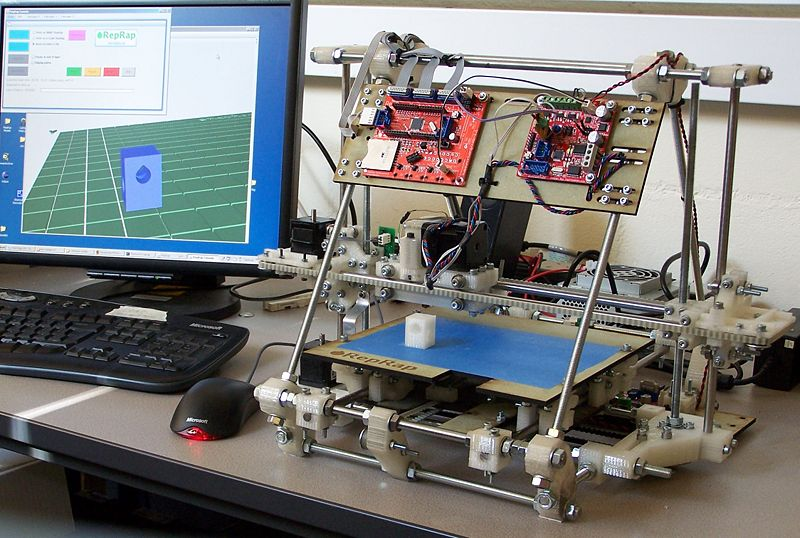
\includegraphics[width=.7\textwidth]{mendel}
	\end{center}
\end{frame}

\begin{frame}
  \frametitle{Directed replication via fabrication}
  \begin{itemize}
  	\item Mechanisms applied to reduce complexity of the prototyper:
  	\begin{itemize}
  	  \item Most of building materials are polylactic acid (PLA);
  	  \item Avoid laser or inkjet print head.
  	\end{itemize}
  	
  	\mbox{ }
  	
  	\item Results :
  	\begin{itemize}
  	  \item Produce up to 57\% of its own part;
  	  \item The number of RepRap machines increased from 4 to 4500 via self-replication (from 2008 to 2011).
  	\end{itemize}
	\end{itemize}
\end{frame}

\subsection{Directed replication via module assembly}

\begin{frame}
  \frametitle{Directed replication via module assembly}
  \begin{itemize}
  	\item A modular robot executes a directed sequence of movement to assemble prepared spare modules to a replica robot.
  	\item Pick and place.
  	
  	\mbox{ }
  	
  	\item Examples :
  	\begin{itemize}
  	  \item Suthakorn \etal\cite{suthakorn_autonomous_2003};
  	  \item Molecubes by Zykov \etal \cite{zykov_self-reproducing_2005}\cite{zykov_evolved_2007};
  	  \item Kaloutsakis and Chirikjian\cite{kaloutsakis_stochastic_2011}.
  	\end{itemize}
	\end{itemize}
\end{frame}

\begin{frame}
  \frametitle{Directed replication via module assembly}
  \begin{itemize}
  	\item Molecubes (from \cite{zykov_self-reproducing_2005}).
	\end{itemize}
	\begin{center}
	  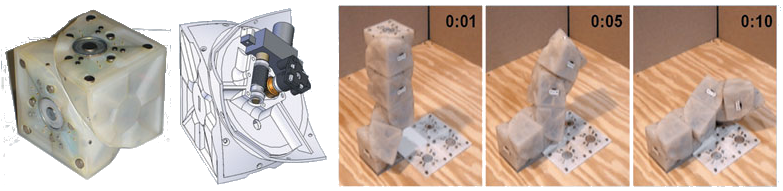
\includegraphics[width=.8\textwidth]{molecubes_a}
	\end{center}
\end{frame}

\begin{frame}
  \frametitle{Directed replication via module assembly}
  \begin{itemize}
  	\item Replication process of a 4-module robot. (from \cite{zykov_self-reproducing_2005}).
	\end{itemize}
	\begin{center}
	  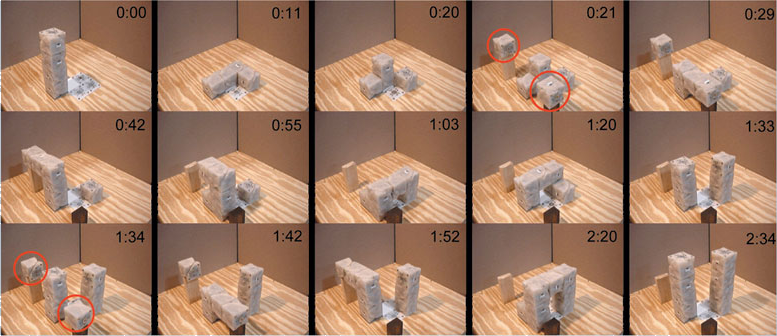
\includegraphics[width=.8\textwidth]{molecubes_b}
	\end{center}
\end{frame}

\begin{frame}
  \frametitle{Directed replication via module assembly}
  \begin{itemize}
  	\item Evolved design of 2-D Molecubes in a simulating environment\cite{zykov_evolved_2007}.
  	\item Two steps:
    \begin{itemize}
      \item Morphology;
      \item Control sequence.
    \end{itemize}
	\end{itemize}
	\begin{center}
	  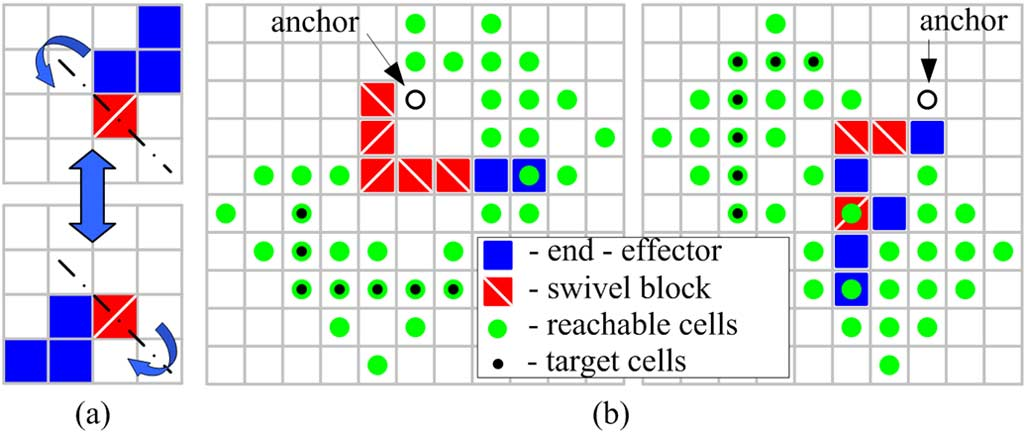
\includegraphics[width=.7\textwidth]{zykov-271}
	\end{center}
\end{frame}

\begin{frame}
  \frametitle{Directed replication via module assembly}
  \begin{itemize}
  	\item Result of evolved design, replication process of an L-shape robot (from \cite{zykov_evolved_2007}).
	\end{itemize}
	\begin{center}
	  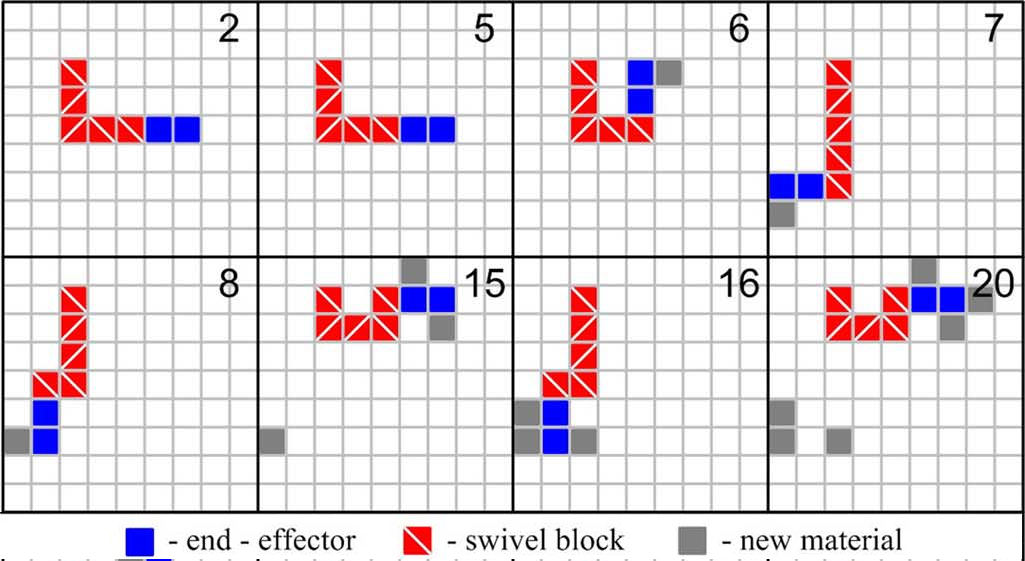
\includegraphics[width=.7\textwidth]{zykov-279-a}
	\end{center}
\end{frame}

\begin{frame}
  \frametitle{Directed replication via module assembly}
	\begin{center}
	  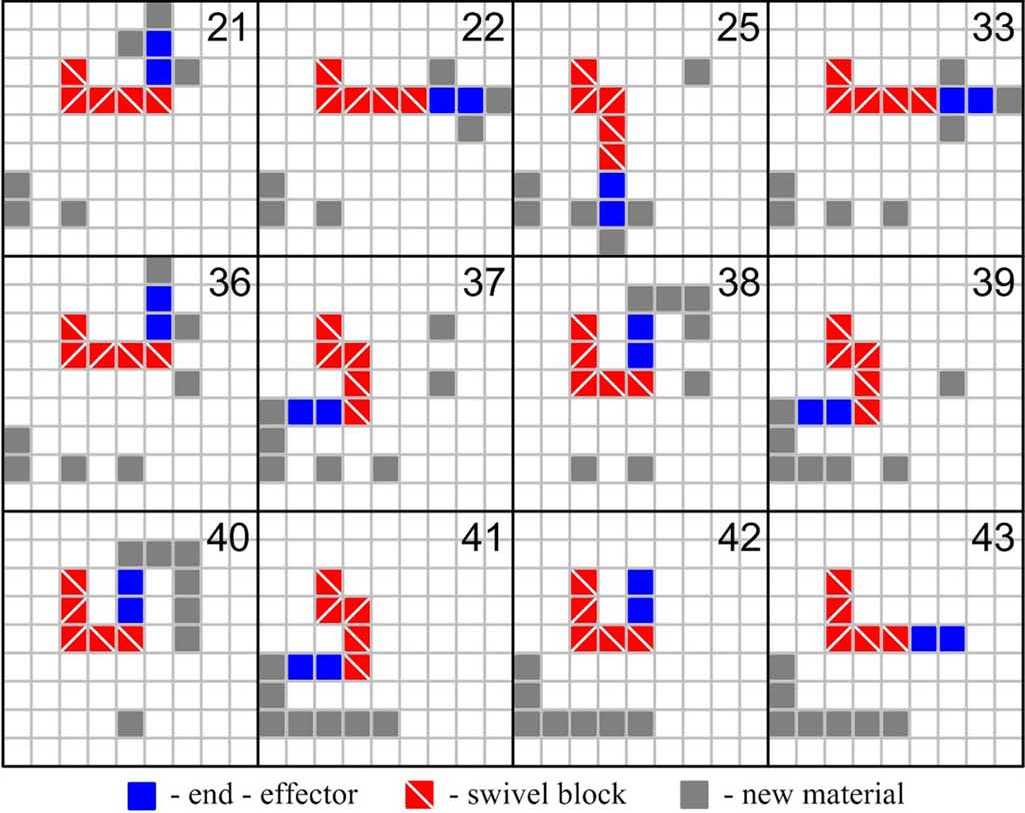
\includegraphics[width=.7\textwidth]{zykov-279-b}
	\end{center}
\end{frame}

\subsection{Self-assembly of randomly agitated modules}
\begin{frame}
  \frametitle{Self-assembly of randomly agitated modules}
  \begin{itemize}
  	\item Modules are kept moving randomly in a environment with external work source, and then assemble to functional parts through a stochastic process.
  	\item Replication of DNA.
  	
  	\mbox{ }
  	
  	\item Examples :
  	\begin{itemize}
  	  \item Penrose\cite{penrose_self-reproducing_1957};
  	  \item Griffith \etal \cite{griffith_growing_2004}\cite{griffith_self-replication_2005};
  	  \item Matsumoto \etal \cite{matsumoto_passive_2009}.
  	\end{itemize}
	\end{itemize}
\end{frame}

\begin{frame}
  \frametitle{Self-assembly of randomly agitated modules}
  \begin{itemize}
  	 \item Electromechanical units in Griffith \etal (from \cite{griffith_growing_2004}).
  	 \begin{itemize}
  	   \item Controlled by 7-state finite-state machine;
  	   \item Able to proofread.
  	 \end{itemize}
	\end{itemize}
	\begin{center}
	  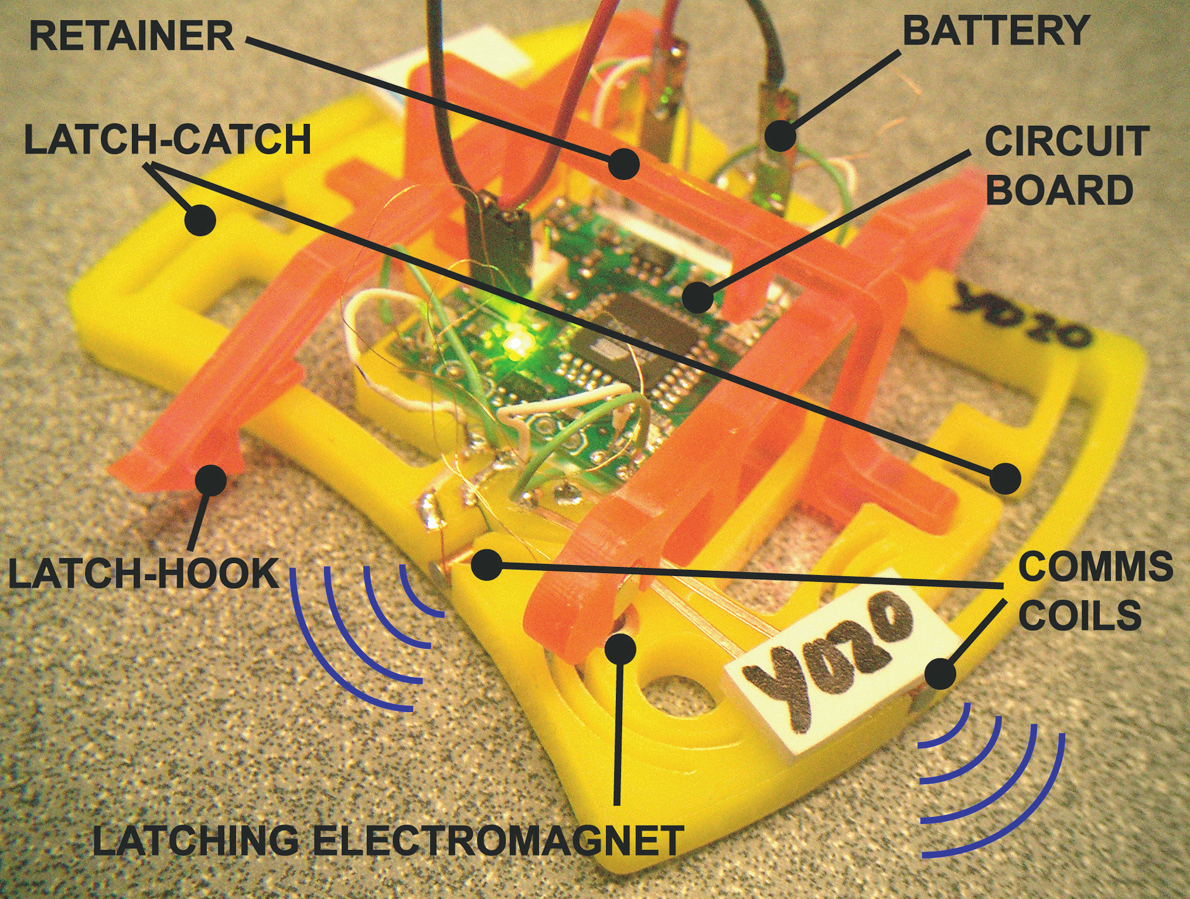
\includegraphics[width=.4\textwidth]{griffith-000} 
	  ~
	  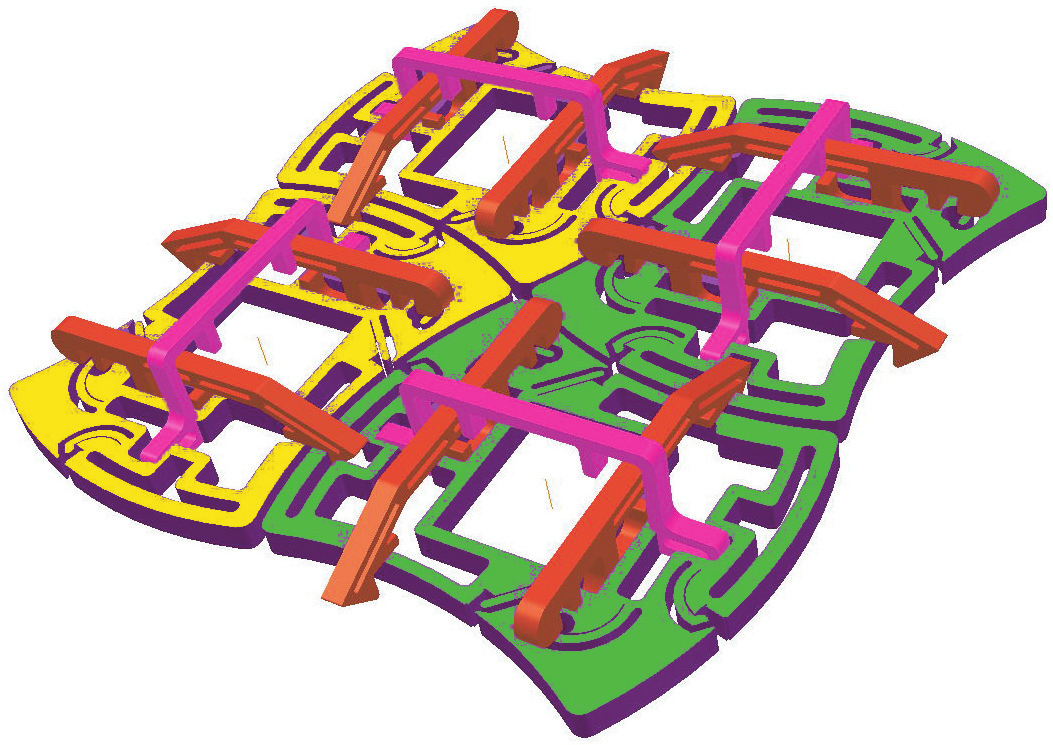
\includegraphics[width=.4\textwidth]{griffith-001}
	\end{center}
\end{frame}

\begin{frame}
  \frametitle{Self-assembly of randomly agitated modules}
  \begin{itemize}
  	 \item Replication process of a 5-bit string (from \cite{griffith_self-replication_2005}).
  	 \begin{itemize}
  	   \item Achieved exponential growth.
  	 \end{itemize}
	\end{itemize}
	\begin{center}
	  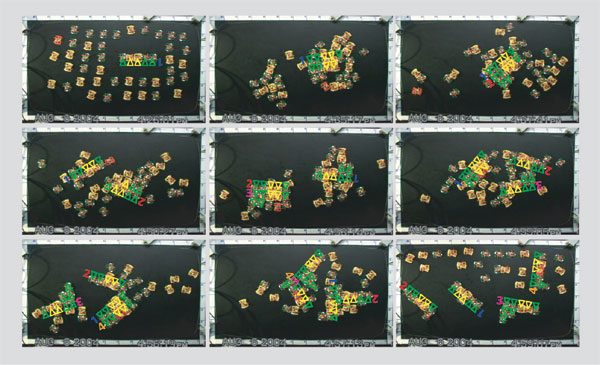
\includegraphics[width=.8\textwidth]{griffith-1}
	\end{center}
\end{frame}

\section{Discussion}
\begin{frame}
  \frametitle{Discussion}
  \begin{itemize}
  	 \item Directed replication via fabrication :
  	 \begin{itemize}
  	   \item Low-complexity input;
  	   \item Dependence on human intervention (assembly);
  	   \item Limitation on fabricating complex components.
  	 \end{itemize}
  	 \item Directed replication via module assembly :
  	 \begin{itemize}
  	   \item Evolved Design;
      \item High-complexity input;
      \item Structured environment.
  	 \end{itemize}
  	 \item Self-assembly of randomly agitated modules :
  	 \begin{itemize}
  	   \item Medium-complexity input;
  	   \item Unstructured environment.
  	 \end{itemize}
	\end{itemize}
\end{frame}

\section{Conclusion}

\frame[t]
{
  \frametitle{Conclusion}

  \begin{itemize}
	  \item Scientists have achieved powerful, practical results in self-replicating robotics.
	  \item Various physically realized self-replicating robots demonstrate the ability of machines to imitate nature organisms from different aspects.
  \end{itemize}

\mbox{ }
  
  \begin{itemize}
  	\item In future, the combination of the different types is possible.
  \end{itemize}
}

%%%%%%%%%%%%%%

\frame[c]{
  \frametitle{The End}
\begin{center}
  Thank you for your attention.\\[1ex]
  Any question?\\[5ex]
\end{center}
}

\section*{References}
\begin{frame}[allowframebreaks]
  \frametitle{References}
  {\footnotesize
  \bibliography{bib}
  \bibliographystyle{plain}  
  }
\end{frame}

\end{document}
